%----------------------------------------------------------------------------------------
% METADATA BLOCK (YAML)  — see inbox/README.md for every field
%----------------------------------------------------------------------------------------
% uid: ""
% school: "lycee"
% level: "4eme"
% section: "Mathématiques"
% chapter: "Coniques"
% title: "L'hyperbole de Kiepert"
% difficulty: "Difficile"
% tags: ["kiepert", "barycentre", "hyperbole-equilatere", "concours", "triangle"]
% provenance: "adapted"
% batch: "2026-11-20-defis-geometrie-A"
%----------------------------------------------------------------------------------------

\newcommand{\R}{\mathbb{R}}

% ---STATEMENT---
Soit $ABC$ un triangle \emph{acutangle et scalène}, de sens direct. On note $a=BC$, $b=CA$, $c=AB$ et
\[S_A=\dfrac{b^2+c^2-a^2}{2},\qquad S_B=\dfrac{c^2+a^2-b^2}{2},\qquad S_C=\dfrac{a^2+b^2-c^2}{2},\qquad S=\det\left(\overrightarrow{AB},\overrightarrow{AC}\right)>0.\]
Pour $\theta\in\left]0,\dfrac\pi2\right[$, on construit à l'extérieur de $ABC$, sur les côtés $[BC]$, $[CA]$, $[AB]$, trois triangles isocèles semblables $A'BC$, $B'CA$, $C'AB$ d'angles à la base $\theta$ (par exemple $\widehat{A'BC}=\widehat{A'CB}=\theta$). On pose $s=\dfrac{S}{\tan\theta}$.

% alt: Triangle ABC, triangles isocèles semblables construits à l'extérieur sur les côtés, droites (AA'), (BB'), (CC') concourantes en K
\begin{center}
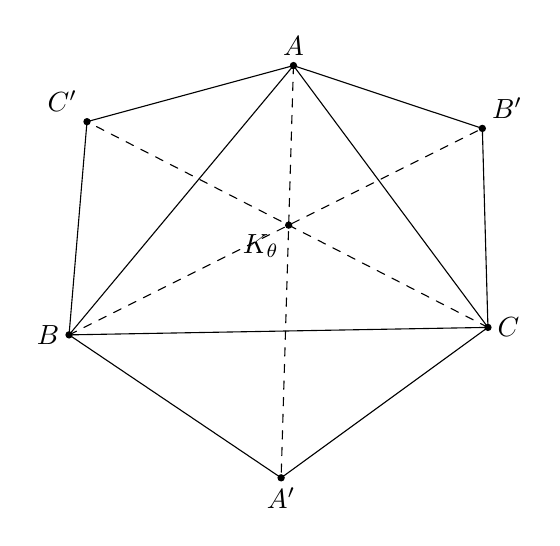
\begin{tikzpicture}[scale=0.95,line cap=round,line join=round,>=stealth]
\draw (0.4,3.2) -- (-2.6,-0.4) -- (3,-0.3) -- cycle;
\draw[thin] (-2.6,-0.4) -- (0.235,-2.311) -- (3,-0.3);
\draw[thin] (3,-0.3) -- (2.925,2.36) -- (0.4,3.2);
\draw[thin] (0.4,3.2) -- (-2.36,2.45) -- (-2.6,-0.4);
\draw[dashed] (0.4,3.2) -- (0.235,-2.311);
\draw[dashed] (-2.6,-0.4) -- (2.925,2.36);
\draw[dashed] (3,-0.3) -- (-2.36,2.45);
\fill(0.4,3.2) circle (1.4pt) node[above] {$A$};
\fill(-2.6,-0.4) circle (1.4pt) node[left] {$B$};
\fill(3,-0.3) circle (1.4pt) node[right] {$C$};
\fill(0.235,-2.311) circle (1.4pt) node[below] {$A'$};
\fill(2.925,2.36) circle (1.4pt) node[above right] {$B'$};
\fill(-2.36,2.45) circle (1.4pt) node[above left] {$C'$};
\fill(0.336,1.067) circle (1.4pt) node[below left] {$K_\theta$};
\end{tikzpicture}
\end{center}

\begin{enumerate}
  \item
  \begin{enumerate}
    \item Montrer que $S_A=\overrightarrow{AB}\cdot\overrightarrow{AC}$ et que $S_B+S_C=a^2$ (et les relations analogues).
    \item Montrer que $A'$ est le barycentre de $(A,-a^2)$, $(B,s+S_C)$, $(C,s+S_B)$ (on pourra décomposer le vecteur $\overrightarrow{MA'}$, où $M$ est le milieu de $[BC]$, sur la base $\left(\overrightarrow{AB},\overrightarrow{AC}\right)$). Écrire les résultats analogues pour $B'$ et $C'$.
  \end{enumerate}
  \item Montrer que \textbf{les droites $(AA')$, $(BB')$, $(CC')$ sont concourantes} en un point $K_\theta$, dont on donnera des coordonnées barycentriques $(x:y:z)$ dans le repère affine $(A,B,C)$.
  \item Soit $\mathcal K$ la conique d'équation barycentrique $(b^2-c^2)yz+(c^2-a^2)zx+(a^2-b^2)xy=0$.
  \begin{enumerate}
    \item Montrer que $K_\theta\in\mathcal K$.
    \item Montrer que $\mathcal K$ passe par $A$, $B$, $C$, par le centre de gravité $G$ et par l'orthocentre $H$ de $ABC$.
  \end{enumerate}
  \item Montrer que \textbf{$\mathcal K$ est une hyperbole équilatère} (on pourra utiliser le fait qu'une conique $\alpha x^2+2\beta xy+\gamma y^2+\cdots=0$ du plan euclidien a ses asymptotes perpendiculaires si et seulement si $\alpha+\gamma=0$).
  \item Réciproquement, montrer que tout point $M(x:y:z)$ de $\mathcal K$ avec $xyz\neq0$ et $M\neq G$ est de la forme $K(s)=\left(\dfrac1{s+S_A}:\dfrac1{s+S_B}:\dfrac1{s+S_C}\right)$ pour un certain réel $s$.
\end{enumerate}

\emph{Remarque.} Les valeurs $s<0$ correspondent aux triangles construits vers l'intérieur. Pour $\theta=\dfrac\pi3$ (triangles équilatéraux), $K_\theta$ est le point de Fermat de $ABC$.

% ---SOLUTION---
\begin{enumerate}[itemsep=14pt]
  \item\leavevmode
  \begin{prop}[Produit scalaire et longueurs]
  \textbf{$\overrightarrow{u}\cdot\overrightarrow{v}=\dfrac{\|\overrightarrow{u}\|^2+\|\overrightarrow{v}\|^2-\|\overrightarrow{u}-\overrightarrow{v}\|^2}{2}$}
  \end{prop}
  \begin{enumerate}[itemsep=8pt]
    \item Avec $\overrightarrow{u}=\overrightarrow{AB}$, $\overrightarrow{v}=\overrightarrow{AC}$ : $\overrightarrow{AB}\cdot\overrightarrow{AC}=\dfrac{c^2+b^2-a^2}2=S_A$.

    Par permutation, $S_B=\overrightarrow{BC}\cdot\overrightarrow{BA}$ et $S_C=\overrightarrow{CA}\cdot\overrightarrow{CB}$.

    $S_B+S_C=\dfrac{c^2+a^2-b^2+a^2+b^2-c^2}{2}=a^2$.

    Deux relations utiles pour la suite, avec $u=\overrightarrow{AB}$, $v=\overrightarrow{AC}$ : $\ u\cdot v=S_A$, $\ \|u\|^2=c^2$, $\|v\|^2=b^2$, d'où
    \[S_A-c^2=\dfrac{b^2-c^2-a^2}{2}=-S_B,\qquad b^2-S_A=\dfrac{b^2-c^2+a^2}{2}=S_C.\quad(\ast)\]

    \item Notons $J$ la rotation vectorielle d'angle $+\dfrac\pi2$ et $t=\tan\theta$, donc $ts=S$.

    Le triangle $ABC$ est direct : l'intérieur est à gauche de $B\to C$, l'extérieur à droite. Le sommet $A'$ est à la hauteur $\dfrac a2\tan\theta$ au-dessus du milieu $M$ de $[BC]$, du côté extérieur :
    \[\overrightarrow{MA'}=-\dfrac t2\,J\left(\overrightarrow{BC}\right).\]

    \begin{prop}[Rotation d'un vecteur dans une base]
    Soient $\overrightarrow{u},\overrightarrow{v}$ non colinéaires, $D=\det(\overrightarrow{u},\overrightarrow{v})$. Alors
    \textbf{$J\overrightarrow{u}=\dfrac{\|\overrightarrow{u}\|^2\overrightarrow{v}-(\overrightarrow{u}\cdot\overrightarrow{v})\overrightarrow{u}}{D}$}\quad et\quad \textbf{$J\overrightarrow{v}=\dfrac{(\overrightarrow{u}\cdot\overrightarrow{v})\overrightarrow{v}-\|\overrightarrow{v}\|^2\overrightarrow{u}}{D}$}.
    \end{prop}
    \emph{Preuve.} Écrivons $J\overrightarrow{u}=\alpha\overrightarrow{u}+\beta\overrightarrow{v}$. Le produit scalaire avec $\overrightarrow{u}$ donne $0=\alpha\|\overrightarrow{u}\|^2+\beta\,\overrightarrow{u}\cdot\overrightarrow{v}$. D'autre part $\det(\overrightarrow{u},J\overrightarrow{u})=\|\overrightarrow{u}\|^2=\beta D$. D'où $\beta=\dfrac{\|\overrightarrow{u}\|^2}{D}$ et $\alpha=-\dfrac{\overrightarrow{u}\cdot\overrightarrow{v}}{D}$. Même méthode pour $J\overrightarrow{v}$.

    Avec $\overrightarrow{u}=\overrightarrow{AB}$, $\overrightarrow{v}=\overrightarrow{AC}$ ($D=S$) et $\overrightarrow{BC}=\overrightarrow{v}-\overrightarrow{u}$, d'après $(\ast)$ :
    \[J\left(\overrightarrow{BC}\right)=\dfrac{(S_A-c^2)\overrightarrow{v}-(b^2-S_A)\overrightarrow{u}}{S}=\dfrac{-S_B\overrightarrow{v}-S_C\overrightarrow{u}}{S}.\]
    Donc $\overrightarrow{MA'}=\dfrac{t}{2S}\left(S_C\overrightarrow{u}+S_B\overrightarrow{v}\right)$. Comme $\overrightarrow{AM}=\dfrac12(\overrightarrow{u}+\overrightarrow{v})=\dfrac{ts}{2S}(\overrightarrow{u}+\overrightarrow{v})$ :
    \[\overrightarrow{AA'}=\dfrac{t}{2S}\Big[(s+S_C)\overrightarrow{AB}+(s+S_B)\overrightarrow{AC}\Big].\]
    Le coefficient de $A$ dans la combinaison barycentrique est
    \[1-\dfrac{t}{2S}(2s+S_B+S_C)=1-\dfrac{2S+ta^2}{2S}=-\dfrac{t}{2S}a^2.\]
    Divisons les trois poids par $\dfrac t{2S}>0$ : \textbf{$A'=\text{bar}\{(A,-a^2),(B,s+S_C),(C,s+S_B)\}$} (somme des poids $2s\neq0$).

    Par permutation circulaire $(A,B,C)\to(B,C,A)$ :
    \[\begin{aligned}B'&=\text{bar}\{(B,-b^2),(C,s+S_A),(A,s+S_C)\},\\ C'&=\text{bar}\{(C,-c^2),(A,s+S_B),(B,s+S_A)\}.\end{aligned}\]
  \end{enumerate}

  \item\leavevmode
  \begin{prop}[Coordonnées barycentriques]
  $M=\text{bar}\{(A,x),(B,y),(C,z)\}$ se note $M(x:y:z)$ (définies à un facteur non nul près).
  Un point de la droite $(AA')$ est un barycentre de $A$ et $A'$ : son poids en $B$ et en $C$ est proportionnel à celui de $A'$. Les points de $(AA')$ sont donc ceux dont les coordonnées vérifient \ib{$y:z=(s+S_C):(s+S_B)$}, car $A'(-a^2:s+S_C:s+S_B)$.
  \end{prop}
  De même, $(BB')$ est l'ensemble des points avec $x:z=(s+S_C):(s+S_A)$ et $(CC')$ celui avec $x:y=(s+S_B):(s+S_A)$.

  Posons $X=s+S_A$, $Y=s+S_B$, $Z=s+S_C$ (tous $>0$ car $ABC$ est acutangle et $s>0$) et
  \[K_\theta=\left(\dfrac1X:\dfrac1Y:\dfrac1Z\right).\]
  Alors $y:z=\dfrac1Y:\dfrac1Z=Z:Y$ : $K_\theta\in(AA')$. De même $x:z=Z:X$ : $K_\theta\in(BB')$, et $x:y=Y:X$ : $K_\theta\in(CC')$.

  Les trois droites sont concourantes en \textbf{$K_\theta=\left(\dfrac1{s+S_A}:\dfrac1{s+S_B}:\dfrac1{s+S_C}\right)$}, point intérieur au triangle (poids positifs).

  \item\leavevmode
  \begin{enumerate}[itemsep=8pt]
    \item Avec $x=\dfrac1X$, $y=\dfrac1Y$, $z=\dfrac1Z$ :
    \[(b^2-c^2)yz+(c^2-a^2)zx+(a^2-b^2)xy=\dfrac{(b^2-c^2)X+(c^2-a^2)Y+(a^2-b^2)Z}{XYZ}.\]
    Le numérateur vaut $s\,[(b^2-c^2)+(c^2-a^2)+(a^2-b^2)]+(b^2-c^2)S_A+(c^2-a^2)S_B+(a^2-b^2)S_C$.

    Le crochet est nul. Reste, en multipliant par $2$ :
    \[\begin{aligned}&(b^2-c^2)(b^2+c^2-a^2)+(c^2-a^2)(c^2+a^2-b^2)+(a^2-b^2)(a^2+b^2-c^2)\\ &\quad=\underbrace{(b^4-c^4)+(c^4-a^4)+(a^4-b^4)}_{=0}-\underbrace{\big[a^2(b^2-c^2)+b^2(c^2-a^2)+c^2(a^2-b^2)\big]}_{=0}=0.\end{aligned}\]
    Donc \ib{$K_\theta\in\mathcal K$}.
    \item \emph{$A$, $B$, $C$ :} $A(1:0:0)$ annule chaque terme (chacun contient deux coordonnées parmi $x,y,z$ dont une nulle) ; idem pour $B$ et $C$.

    \emph{$G(1:1:1)$ :} $(b^2-c^2)+(c^2-a^2)+(a^2-b^2)=0$.

    \emph{$H$ :} montrons que $H=\left(\dfrac1{S_A}:\dfrac1{S_B}:\dfrac1{S_C}\right)$. Soit $P$ ce barycentre. Avec $A$ pour origine, $\overrightarrow{AP}\propto\dfrac1{S_B}\overrightarrow{u}+\dfrac1{S_C}\overrightarrow{v}$ et $\overrightarrow{BC}=\overrightarrow{v}-\overrightarrow{u}$ :
    \[\left(\dfrac{\overrightarrow{u}}{S_B}+\dfrac{\overrightarrow{v}}{S_C}\right)\cdot(\overrightarrow{v}-\overrightarrow{u})=\dfrac{S_A-c^2}{S_B}+\dfrac{b^2-S_A}{S_C}=-1+1=0\]
    d'après $(\ast)$. Donc $(AP)\perp(BC)$ ; par symétrie $(BP)\perp(CA)$ : $P=H$. Le calcul de la question 3a avec $s=0$ s'applique tel quel (le terme en $s$ disparaît) : $H\in\mathcal K$.
  \end{enumerate}

  \item $\mathcal K$ passe par les quatre points $A$, $B$, $C$, $H$. Aucun triple n'est aligné : $A$, $B$, $C$ ne sont pas alignés, et $H$ n'est sur aucun côté car le triangle n'est pas rectangle.

  \begin{prop}[Faisceau de coniques]
  Les polynômes de degré $\le2$ en $(X,Y)$ forment un espace de dimension $6$. S'annuler en quatre points dont trois ne sont jamais alignés impose quatre conditions indépendantes : il reste un plan, engendré par
  $Q_1=\ell_{AB}\,\ell_{CH}$ et $Q_2=\ell_{AC}\,\ell_{BH}$ (produits de deux équations de droites).
  \end{prop}
  Pour $Q_1=(\alpha X+\beta Y+\gamma)(\alpha'X+\beta'Y+\gamma')$, la partie quadratique est $\alpha\alpha'X^2+(\alpha\beta'+\alpha'\beta)XY+\beta\beta'Y^2$, avec $\alpha\alpha'+\beta\beta'=\overrightarrow{n}\cdot\overrightarrow{n}'$ ($\overrightarrow{n}$, $\overrightarrow{n}'$ vecteurs normaux). Or $(AB)\perp(CH)$ et $(AC)\perp(BH)$ : $\overrightarrow{n}\cdot\overrightarrow{n}'=0$ pour $Q_1$ et $Q_2$. Cette condition est linéaire : elle vaut pour toute combinaison, donc pour l'équation de $\mathcal K$ :
  \[\alpha+\gamma=0.\]

  Reste à voir que $\mathcal K$ est une vraie conique non dégénérée. La matrice de la forme $Q(x,y,z)=(b^2-c^2)yz+\cdots$ a pour déterminant $\dfrac14(b^2-c^2)(c^2-a^2)(a^2-b^2)\neq0$ car le triangle est scalène.

  Comme $\alpha+\gamma=0$, le discriminant de la partie quadratique est $\beta^2-\alpha\gamma=\alpha^2+\beta^2$. Il ne peut pas être nul (sinon $\alpha=\beta=\gamma=0$ et l'équation serait celle d'une droite, qui ne peut contenir $A$, $B$, $C$). Donc $\alpha^2+\beta^2>0$ : \textbf{$\mathcal K$ est une hyperbole, à asymptotes perpendiculaires}.

  \item Soit $M(x:y:z)\in\mathcal K$ avec $xyz\neq0$. En divisant l'équation par $xyz$ :
  \[\dfrac{b^2-c^2}{x}+\dfrac{c^2-a^2}{y}+\dfrac{a^2-b^2}{z}=0,\]
  c'est-à-dire $\overrightarrow{m}\cdot\overrightarrow{w}=0$ où $\overrightarrow{m}=(b^2-c^2,\,c^2-a^2,\,a^2-b^2)$ et $\overrightarrow{w}=\left(\dfrac1x,\dfrac1y,\dfrac1z\right)$.

  Le plan $\overrightarrow{m}^{\perp}$ de $\R^3$ contient $\overrightarrow{e}=(1,1,1)$ (car $\sum m_i=0$) et $\overrightarrow{\sigma}=(S_A,S_B,S_C)$ (car $\sum m_iS_i=0$, calcul de la question 3a). Ces deux vecteurs sont indépendants ($S_A\neq S_B$ car $a\neq b$), donc $\overrightarrow{m}^\perp=\text{Vect}(\overrightarrow{e},\overrightarrow{\sigma})$ et
  \[\overrightarrow{w}=\lambda\overrightarrow{\sigma}+\mu\overrightarrow{e}.\]
  Si $\lambda=0$, $\overrightarrow{w}\propto\overrightarrow{e}$ : $M=G$, exclu. Sinon, avec $s=\dfrac\mu\lambda$, $\overrightarrow{w}\propto(s+S_A,s+S_B,s+S_C)$ et $M=K(s)$. $\blacksquare$
\end{enumerate}

\textbf{Remarque.} $s>0$ (triangles extérieurs) ne donne que l'arc intérieur au triangle ; $s\to+\infty$ ($\theta\to0$) donne $G$, $s=0$ ($\theta=\dfrac\pi2$) donne $H$, et $s\to-S_A$ donne $A$. Pour $\theta=\dfrac\pi3$ on retrouve le point de Fermat (résultat classique, admis).

\textbf{Idée :} les coordonnées barycentriques transforment la concourance en une égalité de rapports ; l'équation de $\mathcal K$ devient linéaire en $\left(\dfrac1x,\dfrac1y,\dfrac1z\right)$ et l'hyperbole se paramètre par $s$. Le caractère équilatère vient de ce que $H$ est sur la conique (faisceau de coniques).

\textbf{Piège :} pour un triangle isocèle ($b=c$ par exemple) la conique $\mathcal K$ est dégénérée (une droite : l'axe de symétrie) ; c'est pourquoi on suppose $ABC$ scalène.
